\section*{Dati e risultati}

Il grafico della curva di titolazione da noi ottenuto è riportato in Figura \ref{fig:curva}. Abbiamo quindi ricavato
graficamente il volume $V\ped{eq}$ e il pH del punto di equivalenza. Poichè abbiamo misurato un punto sperimentale che è risultato
essere molto vicino al flesso (si veda grafico della derivata), si è deciso di considerare quel punto come il ``vero''
punto equivalente.

\begin{SCfigure}
    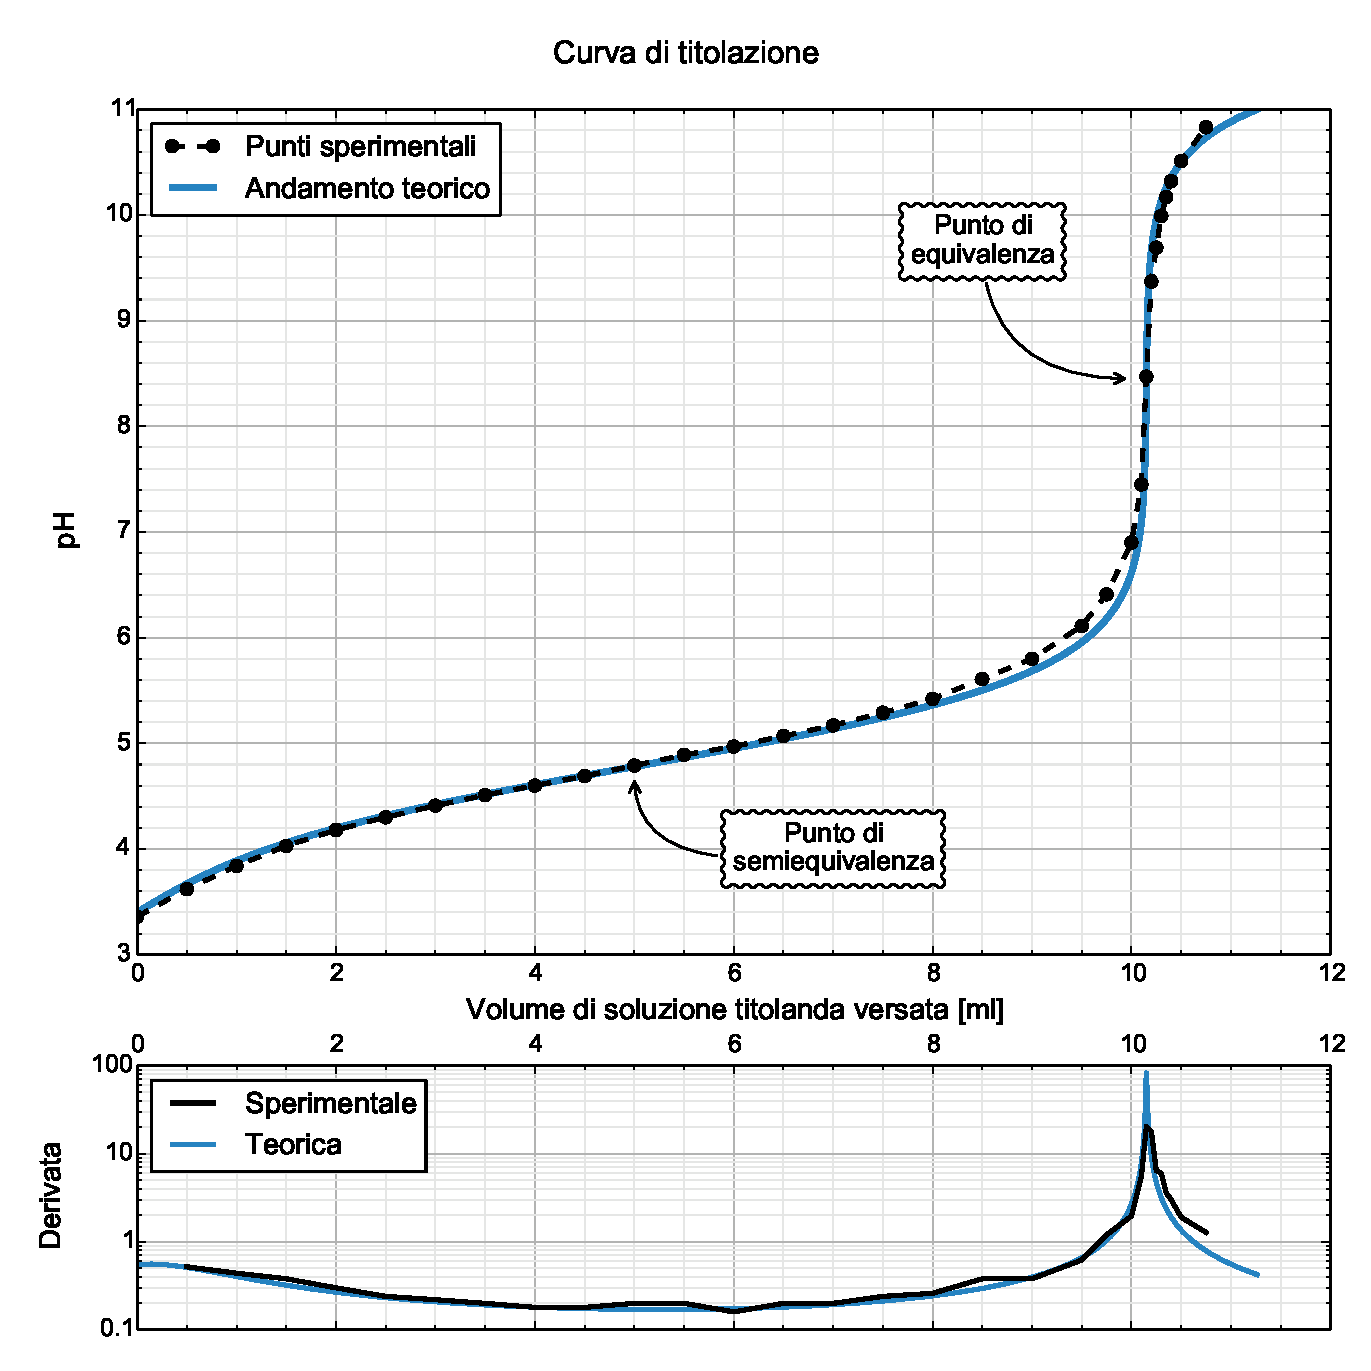
\includegraphics[scale=0.55]{curva.pdf}
    \caption{Le curva di titolazione ottenuta è tipica di un acido debole. Le caratteristiche peculiari sono il punto di equivalenza,
        ovvero il punto in cui il numero di moli di acido e quelle di idrossido sono uguali. Come si vede chiaramente la
        pendenza della curva è massima attorno al punto di equivalenza, fatto che ci permette di individuarlo facilmente grazie al grafico
        della deriva della curva.
        Un altra caratteristica imporante è la zona attorno al punto di semiequivalenza. Questa parte della curva è la
        regione di buffer, dove la soluzione si comporta da tampone, ovvero mantiene il pH circa costante. Infatti la derivata della
        curva è molto piccola. Questo fatto si può sfruttare se è necessario mantenere il pH il più possibile costante, per esempio per le soluzioni
        di taratura del pHmetro. Infine è riportata la curva teorica ricavata dall'equazione \eqref{eq:curv}. Le incertezze non sono riportate
        in quanto non visibili.}
    \label{fig:curva}
\end{SCfigure}

Quindi poichè in quel punto vale $n(\ce{CH3COOH})_i = n(\ce{NaOH})$, si può ricavare il numero di moli di
acido acetico inizialmente presenti e quindi la concentrazione (il volume iniziale era di $V_0 = 100$ ml).

\begin{equation}
    C_0 = \frac{n(\ce{CH3COOH})_i}{V_0} = \frac{n(\ce{NaOH})}{V_0} = \frac{VC}{V_0} = 10.15 \pm 0.04 \; \si{\milli\mol\per\litre}
\end{equation}
%
dove $C = 0.1$ M e $V$ sono rispettivamente la concentrazione e il volume aggiunto della soluzione di \ce{NaOH}.

Occorre notare che questo valore indica la concentrazione $C_0 = \ce{[HAc] + [Ac- ]}$ (per brevità si è indicato l'acetato con \ce{Ac-} e l'acido acetico con \ce{HAc}) presente nella soluzione
e tiene conto del 4\% di acetato già presente all'inizio.

\paragraph{Un semplice calcolo alternativo.}

Similmente a quanto fatto nell'ultimo paragrafo, è possibile ricavare in modo grezzo una stima
della concentrazione conoscendo solo il pH iniziale e la costante di equilibrio, senza
la curva di titolazione.

La formula che ci permette di calcolare la concentrazione si può ricavare impostando il sistema \eqref{eq:sistemone},
che tiene conto delle costanti di equilibrio e dei bilanci di massa e carica.

\begin{equation}
    C_p = \frac{10^{-2 \cdot \text{pH}} + K\ped{A} \cdot 10^\text{-pH}}{K\ped{A}} = 11.39 \pm 0.02 \; \si{\milli\mol\per\litre}
\end{equation}

Il valore ottenuto è simile, anche se non compatibile con quello ottenuto in precedenza.
Esso dà comunque una stima indicativa della concentrazione.

\paragraph{Stima della costante di equilibrio}

I dati che abbiamo ottenuto sono utili per stimare la costante di equilibrio $K\ped{A}$ dell'acido
acetico a temperatura ambiente. Per ricavare questo importante parametro, che abbiamo usato più
volte nella relazione, si sfrutta il punto di semiequivalenza.

Sempre sfruttando il fatto che la reazione \eqref{eq:reaz} può essere considerata stechiometrica,
è interessante considerare cosa accade nel punto $V\ped{eq}/2$. In questo particolare punto,
trascurando la concentrazione iniziale di acetato, si ha che [\ce{CH3COOH}] = [\ce{CH3COO}].
Perciò la legge di azione di massa (prima parte della \eqref{eq:massa}), diventa 

\begin{equation}
    K\ped{A} = \frac{[\ce{Ac-}][\ce{H3O+}]}{[\ce{HAc}]} = [\ce{H3O+}]
\end{equation}

Misurando il pH possiamo ricavare la costante di equilibrio! Abbiamo quindi preso il punto sperimentale
più vicino a $V_0/2$ (abbiamo anche provato a fare un interpolazione lineare tra i due punti più
vicini, ottenendo un risultato identico entro l'incertezza), ottenendo $pK\ped{A} = pH = 4.79$ da cui
$K\ped{A} = 10^{-pH} = (1.62 \pm 0.01) \times 10^{-5}$. Sebbene l'ordine di grandezza del risultato sia corretto, il valore ottenuto non è compatibile con il valore $1.74 \times 10^{-5}$ riportato in letteratura.
Chiaramente la stima dell'incertezza è sottostimata.

\paragraph{Andamento teorico della curva di titolazione.}

È possibile, conoscendo la concentrazione $C_0$, la costante di dissociazione di
acqua e acido acetico e la concentrazione della soluzione titolante,
calcolare a posteriori la curva di titolazione.
Questo si ottiene considerando il seguente sistema di equazioni

\begin{equation}
    \left\{
    \begin{array}{l @\qquad l} \smallskip
        K_w = [\ce{H3O+}][\ce{OH-}] & \text{Protolisi dell'acqua} \\ \smallskip
        K\ped{A} = [\ce{Ac-]}[\ce{H3O+}]/[\ce{HAc}] & \text{Dissociazione dell'acido acetico} \\ \smallskip
        C_0 = \ce{[HAc] + [Ac-]} & \text{Bilancio di massa dell'acido} \\ \smallskip
        CV/(V + V_0) = [\ce{Na+}] & \text{Bilancio di massa dell'idrossido} \\ \smallskip
        \ce{[H3O+] + [Na+] = [OH-] + [Ac-]} & \text{Conservazione della carica} \\
    \end{array}
    \right.
    \label{eq:sistemone}
\end{equation}
%
dal quale si può ricavare la seguente equazione

\begin{equation}
    \frac{CV}{C_0V_0} = \frac{K\ped{A}}{K\ped{A} + \ce{[H3O+]}} + \frac{V + V_0}{C_0V_0} \left(\frac{K_w}{\ce{[H3O+]}} - \ce{[H3O+]} \right)
    \label{eq:curv}
\end{equation}
%
che fornisce la formula della curva di titolazione. In particolare, poichè è difficile isolare la varibile \ce{[H3O+]} in funzione di $V$, essendo
un equazione di $3^\circ$ grado per la prima variabile, è conveniente prendere $V$ come variabile dipendente 
(dall'equazione sopra è facile ricavarla). Per graficare la curva è poi sufficiente tracciarla ad assi invertiti (come $x = g(y)$).
La curva ottenuta è riportata nel grafico in Figura \ref{fig:curva}.

È anche importante notare che dal sistema \eqref{eq:sistemone} si possono ricavare tutte le formula usate nei precedenti paragrafi. Per esempio si può calcolare il rapporto tra acetato e acido acetico all'inizio dell'esperimento. Basta conoscere la costante di equilibrio per l'acido acetico, che a 25$^\circ$C vale
$K\ped{A} = 1.74 \times 10^{-5}$, e il pH iniziale della soluzione, che era 3.36.

\begin{equation}
    K\ped{A} = \frac{[\ce{Ac-}][\ce{H3O+}]}{[\ce{HAc}]} \qquad
    \Longrightarrow \qquad \frac{[\ce{Ac-}]}{[\ce{HAc}]} = \frac{K\ped{A}}{[\ce{H3O+}]} \simeq 4\%
    \label{eq:massa}
\end{equation}
